\chapter{Epoxidation Process}

With the previous chapter, it has been shown that the recirculation of the feed-gas was possible for a gas only plasma system (henceforth referred to as the dry plasma system). While the CO$_2$ dissociation reaction can occur in the previous system,  it cannot produce a useful product. As such this chapter will focus on modifying the dry-plasma system to utilise the atomic oxygen from the CO$_2$ dissociation, by reacting it with a liquid alkene to produce epoxides (henceforth referred to as the wet plasma system). 

\section{Investigation the role of solvent}

As stated in the end of chapter 3, the reaction undertaken in this report builds on the work done by Xu et al \cite{Xu2021}. The co-reactant used for this reaction would be trans-Stilbene, which utlises the atomic oxygen produced in the CO$_2$ dissociation to produce the epoxide called trans-Stilbene oxide (which are used interchangeably for the rest of this report). 

One thing to note is that trans-Stilbene is a crystalline solid. Thus in the work done by Xu et al \cite{Xu2021}, it was dissolved in a solvent; specifically acetonitrile. This is a common solvent used in chemistry for organic synthesis due to its high solvent power, especially for dissolving organic compounds. Additionally, its low viscosity and high chemical stability make it very useful when it comes to gas chromatography. 

While the aforementioned benefits make it ideal for facilitating the epoxidation process, there are several drawbacks to using it. The most significant drawback is that due to its high solvent power, it tends to attack most plastics, rubbers, and even some types of coatings. The reason this is a problem is that many of the components used for designing the dry plasma system, which include the mass flow controllers and pressure sensors, all use seals that are mode from FKM (a fluorocarbon-based synthetic rubber). As such, if those seals are exposed acetonitrile for a prolonged period, it would cause softening and/or swelling of those seals, leading to a potential failure of the part. This tends to be less of an issue in an open gas loop configuration, where most of the gases are vented into atmosphere. However, this issue is particularly significant in a closed gas loop system, where the gases are recycled and any acetonitrile that evaporated into the gas phase would accumulate over time as the system was run.

Another downside with using acetonitrile as the solvent is that is typically classed as a non-green solvent.``Green" solvents is a loose term to describe solvents that minimise the impact on the environment. As such, green solvents are typically expressed on a spectrum as all solvents typically have some impact on the environment throughout its life cycle, and also have potential hazards in the early stages of producing the chemical compounds. The conventional example of a green solvent commonly used in industry is ethanol.

\begin{figure}[h!]
	\centering
    \includegraphics[width=0.85\linewidth]{chapter_6/figures/green_solvent.png} 
	\caption{Environmental assessment of 26 of the most common organic solvents used done by Capello et al \cite{}.}
	\label{fig:green_solvent}
\end{figure} 

A useful illustration of this concept can be seen in figure \ref{fig:green_solvent}, which shows the environmental assessment of several of the most popular solvents used. This work, done by Capello et al \cite{Capello2007}, compares the environmental, health, and safety (EHS) score of the solvents (which are assessed on a points basis, where a lower score indicates a safer solvent) against the life-cycle assessment (LCA) score of the solvents (which evaluates the cumulative energy demand for producing a solvent and recycling or incinerating it once used, where a lower score indicates a for energy efficient solvent). As seen in the figure, acetonitrile is one of the worse solvents evaluated.

The relevance of this concept of green solvents is that one of the aims of this research is to asses the feasibility of scaling up this epoxidation process to industry. As such it would be prudent to first investigate the role of the solvent in producing the epoxide, as the feasibility of using a greener solvent would make a more compelling case for scaling up the process. 

For this evaluation, a much smaller set of solvents were tested, simply due to availability of the solvents in the laboratory. In addition to acetonitrile, these include ethanol, iso-propanol, and acetone. The important point to note here is that all the chosen solvents were classed as ``greener" than acetonitrile in the assessment criteria developed by Capello et al \cite{Capello2007}. 

To evaluate this, the plasma was generated using COST jet. The reason for reverting to the COST jet over the SRR jet for this experiment was to simply eliminate potential variables. Since the COST jet had been previously used for the epoxidation reaction, this would give a good reference for comparing the solvents used. Additionally, the COST jet could be used a basis to design the reactor for the wet plasma system.

As for the experimental setup, a 1\% CO$_2$+He gas mixture was used. The COST jet was set to operate at approximately 10 W, which was the minimum power that would sustain the plasma with the chosen gas mixture. The nozzle of the jet was placed approximately 5-10 mm above the surface of the treated liquid. As for the treated liquid, it was a 10 mM solution of trans-Stilbene in the tested solvent, with 10 mL of solvent used. The treated liquid was placed in an ice bath, to keep the temperature at approximately 0 C. The liquid was then treated for a span of 2 hours. These experimental conditions were chosen to mimic the ones done by Xu et al \cite{Xu2021} as close as possible.

With these experiments run, four samples were produced. To evaluate the composition of these samples, the method chosen was the gas chromatography–mass spectrometry (GC-MS). As the name suggests, the method combines the techniques of gas chromatography and mass spectrometry to separate different compounds in a sample and identify them. 

The first stage of a GC-MS test is the gas chromatography portion, where the injected compounds are vaporised. The vaporised compounds are then moved through the device the aid of a carrier gas, which is typically an inert gas such as helium though other non-reactive gases such of nitrogen can also be used. Regardless of the gas chosen, it carries the vaporised sample through a column. The column is essentially a narrow tube with an inner coating that is called the stationary phase. The substances in the sample interact with the stationary phase differently based on their chemical and physical properties, as such will travel through and exit the column at different rates.

The substances exiting the column (which would typically be a single compound assuming that the procedure for the GC-MS was set up correctly) then enters the mass spectrometer. Once they enter the mass spectrometer, they first gets ionised to give them a charge. These newly formed ions then get accelerated to the same velocity before being deflected by a magnetic field. The amount of deflection of the ions depends on two factors: their mass and charge. The lighter the mass of the ion, the greater the deflection. Similarly, the larger the charge of the ion, the more they deflect. Ions with the same mass-to-charge ration would experience the same deflection, which are then measured by the detector. An illustration of the gas chromatogram and mass spectrometer schematics are shown in figure \ref{fig:GC-schematic} and \ref{fig:MS-schematic} respectively. \\

\begin{figure}[h!]
	\centering
    \includegraphics[width=0.8\linewidth]{chapter_6/figures/GC-schematic.png} 
	\caption{A schematic diagram of the gas chromatography method \cite{PerkinElmer2022}.}
	\label{fig:GC-schematic}
\end{figure} 

\begin{figure}[h!]
	\centering
    \includegraphics[width=\linewidth]{chapter_6/figures/MS-schematic.jpeg} 
	\caption{A schematic diagram of the mass spectrometry method \cite{Aryal2022}.}
	\label{fig:MS-schematic}
\end{figure} 

The GC-MS used was the Shimadzu GCMS-QP2010 Ultra. It was equipped with a [insert name here] capillary column (30 m × 0.25 mm × 0.25 $\mu$m). The samples were injected into the GC-MS with a with a configured split ratio of 10:1, and an injected volumne of 1 $\mu$L. A helium carrier gas used was fed in at a constant flow rate of 65 mL/min. As for the procedure used, the column was at 50 $^{\circ}$C for 5 minutes, then increased to 300 $^{\circ}$C at a rate of 20 $^{\circ}$C/min and finally held there for 5 additional minutes. Thus, the total run time per sample was 23 minutes. 

The results of these solvent comparisons are shown in figures \ref{fig:solvent_test_results}. From the data it was clear that the best performing solvent was in fact acetonitrile, followed by acetone. The possible reason for this is that the vapour pressure for acetone was approximately 3 times larger than that of acetonitrile, meaning that there was significantly more evaporation, which in turn meant that it was difficult to keep a consistent distance between the nozzle of the jet and the surface of the liquid. As for both the alcohols, they performed very poorly with ethanol marginally producing more trans-stilbene oxide over the iso-propanol. The reason for this is unclear, though it is most likely explanation for this behaviour is that the atomic oxygen produced would react with the alcohols, oxidising them. However, preliminary testing with a basic gas chromatography detector failed to find the by products which would be produced from this oxidative reaction. As such further research needs to be undertaken to understand this behaviour, which was unfortunately beyond the scope of this project.

\begin{figure}
    \centering
    \begin{subfigure}[b]{\textwidth}
        \centering
        \includegraphics[width=\textwidth]{chapter_6/figures/solvent_test.png}
        \caption{}
        \label{fig:solvent_test}
    \end{subfigure}
    \hfill
    \begin{subfigure}[b]{\textwidth}  
        \centering 
        \includegraphics[width=\textwidth]{chapter_6/figures/solvent_test_close_up.png}
        \caption{}
        \label{fig:solvent_test_close_up}
    \end{subfigure}

    \caption{\small A wide (a) and close-up (b) illustration of the GC-MS results from testing the reaction of atomic oxygen with trans-Stilbene dissolved in different solvents.} 
    \label{fig:solvent_test_results}
\end{figure}

Another thing to note was the large presence of benzaldehyde for the reactions with the acetonitrile solvent. Benzaldehyde is typically only formed when trans-Stilbene reacts with ozone. The source of this ozone had to have come from the surrounding air around the testing container. As such, the container was sealed off and tested again. The results shown in figure \ref{fig:open_vs_closed_cost_jet_results} show a significant reduction in this peak, confirming that a sealed reactor was necessary for the reaction of trans-Stilbene.

\begin{figure}
    \centering
    \begin{subfigure}[b]{\textwidth}
        \centering
        \includegraphics[width=\textwidth]{chapter_6/figures/open_vs_closed_cost_jet.png}
        \caption{}
        \label{fig:open_vs_closed_cost_jet}
    \end{subfigure}
    \hfill
    \begin{subfigure}[b]{\textwidth}  
        \centering 
        \includegraphics[width=\textwidth]{chapter_6/figures/open_vs_closed_cost_jet_close_up.png}
        \caption{}
        \label{fig:open_vs_closed_cost_jet_close_up}
    \end{subfigure}

    \caption{\small A wide (a) and close-up (b) illustration of the GC-MS results from testing an open and closed container of the reaction of trans-Stilbene in acetonitrile. Note, the naphthalene peak was due to its introduction as an internal standard.} 
    \label{fig:open_vs_closed_cost_jet_results}
\end{figure}

From these experiments, the unfortunate conclusion was that acetonitrile had to be used as the solvent of choice for the reactor. This meant that the experiment setup used needed to include some mechanism to remove acetonitrile that was kicked up into the gaseous phase by the SRR jet blowing on the liquid. The design of the reactor and the process of removing the acetonitrile gas are described in the next section.

\pagebreak

\section{Developing the plasma reactor}
\subsection{Designing the main reactor housing}

From the usage of the COST jet, several key design requirements were obtained for the  design of the SRR jet reactor. These requirements and the rational for them are detailed in the list below.

\begin{itemize}
    \item \textbf{The reactor housing needed to be completely enclosed}: The main reason for this was that the end goal of the system designed was to function in a closed gas loop configuration. Hence, an enclosed reactor housing that is as leak proof as possible would minimise the feed gas required to top up the system. Additionally, from the previous tests with the COST jet, it was determined that any air present in the system would oxidise the atmospheric oxygen into ozone, in turn reducing the overall yield of the reaction.
    
    \item \textbf{The surface of the treated liquid needed to be as close as possible to the SRR jet}: This was because the atomic oxygen produced in the decomposition by the plasma is a very short lived species, reacting with anything it comes into contact with. Thus, being able to bring the surface of the liquid as close as possible to the jet would increase the carbon dioxide efficiency of the system, and should also produce an increase in yields. This distance is a key discussion topic in this chapter, and will be henceforth referred to as the \textit{reaction distance}.
    
    \item \textbf{The gas outlet of the reactor housing needed to be small}: This is a byproduct of the previous requirement of minimising the reaction distance. As such, the tube to allow the gas flow out of the housing needed to be kept small as well. 
    
    \item \textbf{There needed to be an inlet for introducing the liquid into the reactor}: The reason for this was to do with the fact that gas blowing on the surface of the liquid increases the rate of evaporation of the solvent. This mechanism in turn increases the reaction distance over time. As such, there needed to be an inlet to allow for topping up the solvent, ensuring that reaction distance remained constant. 
\end{itemize}

Armed with these requirements, several prototype reactor housings were made. From those designs, several additional findings were learnt. Firstly, the early prototypes designed included a design where the gas from the plasma was bubbled into the liquid rather than simply reacting with the surface of the liquid. The idea was to increase the mixing of liquid and potentially promoting an increase in the the rate of reaction. However, this idea was eventually scrapped because it significantly increased the rate of evaporation of the solvent, meaning that it was more difficult to keep the reaction distance constant. Additionally, the splashing generated would mean that liquid would escape from the reactor and into the gas outlet of the reactor, which would not be easily recoverable at the end of the experiment.

Another learning from the prototypes was with regards to the reservoir of the reactor housing. One of the prototypes made consisted of a multi reservoir design, where the main reactor would contain a small liquid reservoir, while a larger reservoir was kept separate and connected using some tubing and a peristaltic pump. The reasoning for this was that larger volumes of liquid trans-Stilbene could be used, which was inline with how large scale industrial chemical reactions occur. While this idea did work, it was somewhat inconsistent mainly due to the fact that maintaining a constant reaction distance proved challenging with only the use of a single peristaltic pump. This was because the tubing of the inlet and outlet from the larger to the smaller reservoir stretch slightly differently in the pump, meaning that there was very small but noticeable difference in the liquid flow rates. This in turn meant that the liquid volume in the smaller reservoir (within the reactor) would either increase or decrease due to this flow discrepancy. While this is a solvable problem, either with the use of an additional peristaltic pump or a liquid level sensor and some PID controllers, it was decided that this was scope for a future research project and hence was removed. 



\begin{figure}
    \centering
    \begin{subfigure}[b]{0.475\textwidth}
        \centering
        \includegraphics[width=\textwidth]{chapter_6/figures/SRR_jet_reactor_schematic.png}
        \caption{}
        \label{fig:SRR_jet_reactor_schematic}
    \end{subfigure}
    \hfill
    \begin{subfigure}[b]{0.475\textwidth}  
        \centering 
        \includegraphics[width=\textwidth]{chapter_6/figures/SRR_jet_reactor_schematic.jpeg}
        \caption{}
        \label{fig:SRR_jet_reactor_picture}
    \end{subfigure}

    \caption{\small An illustration of the schematic design (a) and finished SRR jet  reactor build (b).} 
    \label{fig:SSR_jet_reactor_illustration}
\end{figure}

With those additional findings, the final reactor schematic and build are shown in figure \ref{fig:SSR_jet_reactor_illustration}. The reactor housing is comprised of 4 different parts. The main housing containing the liquid was simply a repurposed glass sample bottle. This was then connected to a short piece of stainless pipe, functioning as a coupler between the glass and the base of the SRR ground plane. The stainless steel coupler also contained two holes to allow for the inlet and outlet glass tubing. The inlet tube was bent 90 degrees and extended to the bottom of the glass sample bottle, while the outlet tube was simply placed at the top of the stainless steel coupler. All the components were the then bonded together with the use of Torr Seal\textsuperscript{\tiny{\textregistered}} epoxy, which is a two part epoxy designed for low pressure applications. Then the finished reactor housing was attached to the SRR ground plane using superglue. The reason for this was that the epoxy would not attach to the gold plated coating on the ground plane SRR PCB.

Due to the use of acetonitrile as a solvent, there were only three realistic options for designing the housing. These include some form of metal (preferably stainless steel due to its corrosion resistance in the presence of oxygen), a plastic that has a high chemical resistant to acetonitrile (such as PTFE), or glass. Each of these options had their respective benefits and drawbacks. Stainless steel would provide excellent thermal dissipation in order to cool the reactor housing, and would be easy to machine; however it is opaque so observing the reaction distance would not be possible, and stainless steel is quite heavy meaning that the reactor would need additional support. PTFE would also easily machinable and could be made translucent, allowing for the viewing of the reaction distance; but is an insulator and due to its chemical resistance, difficult to bond with other components. Glass is transparent, allowing for easy observations of the reaction distance, and has a thermal conductivity in between stainless steel and PTFE; though it had the disadvantage of being relatively difficult to machine. As such, a compromise was stuck to use a combination of glass and stainless steel, minimising the shortcomings of each material on their own.

The glass tubing used was the smallest tubing available in the laboratory, with an outer diameter of 4.3 mm. However, in order to make drill holes for the glass tubing through the stainless steel coupler, it needed to be slightly wider than the outer diameter of the tubing. As such, the coupler was designed to be 8mm thick, which would be the theoretical minimum reaction distance. In practice, this distance was slightly longer at approximately 10 mm, due to the tapering walls present the glass bottle. As such, the maximum volume of the reactor was around 12 mL of liquid. 

\subsection{Removing the acetonitrile vapours}

As stated earlier in this chapter, the gas blowing from the SRR jet onto the surface of the liquid would increase the rate of evaporation of the acetonitrile solvent. This effect could be minimised by either reducing the flow rate of the SRR jet or decreasing the temperature of the liquid, but neither approach would completely eliminated this phenomenon. The evaporation causes the presence of acetonitrile vapour in the system, which as mentioned previously would have a detrimental effects on various components within the system. As such it was vital to attempt to eliminate as much acetonitrile vapours as possible. In chemistry, this is typically achieved using a condenser to cool the acetonitrile in the gas phase back to a liquid. The general principle of a condenser is the cooling liquid surrounding the condenser has to have a lower temperature than the boiling point of the substance being condensed. 

However, the use of a traditional condenser in this application would not be particularly feasible. This was primarily due to the constant circulation of the gas within the system, meaning that the duration the gas spends in the condenser was governed by the flow rate of the gas. Thus depending on the flow rate used, there would be an insufficient amount of time for most of the acetonitrile to condense back into its liquid form. This could be solved in one of two ways. Firstly, one could increasing the duration the gas spends in the condenser by either using a very long condenser tube, a similar concept to the condenser coils on refrigerator; or by increasing the number of condenser tubes in parallel, a method used in surface condensers typically found in power stations to cool exhaust gases from the turbine. The issue with either of these methods was that they would increase the volume of gas in system. Specifically, it would increase the volume of gas within the main reaction chamber which is kept at atmospheric pressure by the PI controller. The reason this is a problem is that it would increase the lag time of the system, thus the PI controller used would not work to maintain the pressure of the main chamber.

The other solution for the condenser would be to cool the gas as fast as possible, resulting in as much acetonitrile to be drawn out of the gaseous state. The benefit of this method is that the condenser does not have to be particularly large, thus the controller designed in the previous chapter would sufficiently work. However this was where the first issue lied, as acetonitrile has a melting point of -45 $^{\circ}$C. This meant that a traditional lab condenser would not work as those rely on circulating water through an ice bath, keeping the condenser at just above 0 $^{\circ}$C. The obvious next step was to then use an alternative condenser design, and the one chosen was called the direct-contact condenser. This design directly mixes the gas with the cooling liquid, forcing the gaseous acetonitrile to give up its latent heat and condense with the cooling liquid. Nonetheless, the challenge would be keeping the cooling liquid to -45 $^{\circ}$C. The two options for this would be to either changing the pressure of the condenser, thus altering the melting point of acetonitrile; or use solid acetonitrile to cool the cooling liquid. However, the changing the pressure of the condenser was not viable since the reactor has to be at atmospheric pressure, and using large amounts acetonitrile being cooled to its solid state would be quite expensive. 

Instead the solution was to take the temperature of cooling liquid beyond the melting point of acetonitrile. This would be much easier achieved by simply using ethanol as the cooling liquid (which has a melting point of -114 $^{\circ}$C). The ethanol could be kept cool using some dry ice placed externally to the condenser. The resulting approach would keep the cooling liquid at around -60 to -70 $^{\circ}$C. As such, this lead to the direct-contact condenser design used, shown in figure \ref{fig:condenser_design_1}. The exhaust gas from the reactor would enter the condenser via a stainless steel tube, then the gas was bubbled directly through the cool ethanol, before it escaped though an outlet to the mass flow controller regulating the pressure in the main chamber. 

However, this design introduced a new problem, in which the condenser would perform too well. Due to the extremely cool temperature of the cooling solution, the gaseous acetonitrile does rapidly to a liquid, but then continues to cool to become a solid. Since the gas brought into the condenser entered through the stainless steel tube, this was the first point at which the solid acetonitrile formed (along the walls of the tube). Over time this solid built up, eventually clogging the tube. This resulted in a blockage, thus no gas could enter the condenser; which in turn caused the  pressure in the reactor to rise since there was no outlet for the exhaust gas. 

To solve this, the tube needed to be kept as warm as possible to prevent the solid build up of acetonitrile, but cool enough that it did not interfere with the temperature of the cool ethanol of the condenser. This was achieved by adding a heating element within the inlet stainless steel tube. The heating element was made from nichrome wire, a component commonly found in hairdryers. The nichrome wire was shielded in some thin PTFE tubing to prevent any contamination of the recirculated gases or the cooling liquid. The wire was connected to an external DC power supply, and the current through the nichrome wire was set to approximately 0.5 A. This number was simply chosen via trial an error, though the exact temperature of the inlet stainless steel tube remained an unknown due to the inability to attach a thermocouple since the design of the condenser needed to be air-tight. 

Additionally, a valve was added to the inlet of the condenser to allow a separation between the main reactor chamber and the condenser. This was to allow the reactor to be drawn to a vacuum in order to ignite the plasma and ensure that the gas composition in the reactor is purely Helium. The finalised condenser design can be seen in figure \ref{fig:condenser_design_2}.

\begin{figure}
    \centering
    \begin{subfigure}[b]{0.475\textwidth}
        \centering
        \includegraphics[width=0.8\textwidth]{chapter_6/figures/condenser_design_1.png}
        \caption{}
        \label{fig:condenser_design_1}
    \end{subfigure}
    \hfill
    \begin{subfigure}[b]{0.475\textwidth}  
        \centering 
        \includegraphics[width=0.8\textwidth]{chapter_6/figures/condenser_design_2.png}
        \caption{}
        \label{fig:condenser_design_2}
    \end{subfigure}
%    \vskip\baselineskip
%    \begin{subfigure}[b]{0.475\textwidth}   
%        \centering 
%        \includegraphics[width=0.6\textwidth]{chapter_6/figures/condenser_design_2.png}
%        \caption{}    
%        \label{fig:condenser_build}
%    \end{subfigure}

    \caption{\small An illustration of the schematic design of the direct-contact condenser (a) and the finalised direct-contact condenser with a nichrome heating element (b).} 
    \label{fig:condenser_design_both}
\end{figure}

\subsection{Complete setup design}

With the addition of the addition of the reactor and the condenser, it would be useful to have an updated visualisation of the experimental setup. This is shown in figure \ref{fig:complete_reactor_schematic}. 

\begin{figure}[h!]
	\centering
    \includegraphics[width=\linewidth]{chapter_6/figures/reactor_schematic.png} 
	\caption{An illustration of the completed SSR jet reactor schematic used as the experimental setup.}
	\label{fig:complete_reactor_schematic}
\end{figure} 

On top of the new aforementioned components, an additional mass flow controller was added (shown as MFC$_5$) for venting the gases into atmosphere rather than recirculation. This was done for two reasons. Firstly, because of the addition of the condenser, it was no longer possible to pull the entire system to a vacuum. As such, in order to ensure a pure gas composition in the overall system, it is necessary to perform an initial flushing process. The second reason was for a matter of convenience, as most of the characterisation of the SRR jet reactor (seen in the next section) was done in an open loop gas configuration; thus, this allows the system to be run in both an open and closed gas loop configuration. The details for the control mechanism for this additional mass flow control are not necessarily pertinent in this chapter, however it essentially toggles between the venting mass flow controller (MFC$_5$) or the recirculation mass flow controller (MFC$_3$) based on an open gas loop or closed gas loop configuration respectively.


\section{Characterising the plasma reactor}

With the plasma reactor designed, and the full system operational, the next steps were to characterise the reactor to evaluate the best conditions to run it in. This would be done by changing a parameter at a time, then running the plasma over the trans-Stilbene solution a two hour period of time, and finally running the product through a GC-MS for quantification.

However, in order to obtain quantitative results from the GC-MS, one needs a calibration curve for the starting material (in this case trans-Stilbene) and the final product (which is the trans-Stilbene oxide). To run this, several 0.5 mL solutions of trans-Stilbene and trans-Stilbene oxide were made, each with a different concentration. Then an internal standard was added, which in this case was 50 $\mu$L of Naphthalene with a concentration of 200 mM. The concentrations of trans-Stilbene run were: 10mM, 5 mM, 2.5 mM, 1.25 mM, 1 mM, and 0.5 mM. As for the trans-Stilbene oxide, two additional runs were done so the concentrations were: 10mM, 5 mM, 2.5 mM, 1.25 mM, 1 mM, 0.5 mM. 0.25 mM, and 0.125 mM. The reason for this was because amount of epoxide produced was going to be much smaller than the amount of starting material used. 

\begin{figure}
    \centering
    \begin{subfigure}[b]{\textwidth}
        \centering
        \includegraphics[width=\textwidth]{chapter_6/figures/calibration_curve_ts.png}
        \caption{}
        \label{fig:calibration_curve_ts}
    \end{subfigure}
%    \hfill
    \begin{subfigure}[b]{\textwidth}  
        \centering 
        \includegraphics[width=\textwidth]{chapter_6/figures/calibration_curve_tse.png}
        \caption{}
        \label{fig:calibration_curve_tse}
    \end{subfigure}

    \caption{\small The calibration curve of trans-Stilbene for molar concentrations between 10 mM to 0.5 mM (a) and trans-Stilbene epoxide for molar concentrations between 10 mM to 0.0125 mM (b).} 
    \label{fig:calibration_curve}
\end{figure}


With these samples run in the GC-MS, the area under the desired peaks were integrated. For the internal standard, the peak was located after 8.75 minutes, with the trans-Stilbene peak located at 11.21 minutes and the trans-Stilbene oxide located at 11.25 minutes. For the calibration curve, the ratio of the reference material (either trans-Stilbene or trans-Stilbene oxide) to the internal standard was taken. These are shown in figures \ref{fig:calibration_curve_ts} and figure \ref{fig:calibration_curve_tse} for  trans-Stilbene and trans-Stilbene oxide respectively.

In addition to the calculated ratios, an equation for a regression line was determined based on the provided points. These equations are shown in the figures. Both regression lines fitted strongly to the GC-MS measurements, where the calibration curve of trans-Stilbene had a R2 score of 0.997, while trans-Stilbene oxide had a R2 score of 0.998. These equation of regression were used to determine the concentration of trans-Stilbene spent and trans-Stilbene oxide produced for all subsequent experiments.

\subsection{Evaluating impact of flow rate and reaction distance}

The first set of characterisation tests performed were in relation to the flow rate of the gas through the orifice of the SRR jet, which was arguably the most important of the tests to be performed. This is because, the speed at which the atomic oxygen strikes the trans-Stilbene solution, and the frequency of this occurrence are governed by the flow rate. 

In the previous chapter, a lot of the initial characterisation of the SRR jet for the controller design of the dry plasma system were done with flow rates of up to 50 sccm. However, the the SRR jet was capable of signficantly higher flow rates. As such, for these set of experiments, a range of flow rates between 100 sccm to 2000 sccm or simply 2 slm (which refers to standard litres per minutes) were tested. However there was a slight complication that occurred while running these tests. This is because, as the flow rates were increased, one could no longer continue maintaining the smallest possible reaction distance due to the strong jet essentially splashing the liquid. This splashing was an issue as it allowed the liquid to escape through the gas outlet of the reactor, meaning an irrevocable loss of the yields produced by the epoxidation process. As such, as the flow rates were increased the reaction distance also had to increase. Nonetheless, for the sake of being able to ascertain the impact of reaction distance for the given flow rate, additional runs at said flow rate were performed while varying the reaction distance. 

For these runs, there were only two variables being changed were the flow rate and reaction distance, all other parameters were kept constant. These parameters included the pressure being kept at 760 Torr, the CO$_2$-He concentration being kept at a 1\% mixture, the temperature of the liquid being kept at approximately 0 $^{\circ}$C using an ice bath, and most importantly the power of the plasma kept at 10 W (the same as the runs with the COST jet). 

As for the experimental procedure, the tests were run continuously over the course of two hours. The samples were a 12 mL solution of trans-Stilbene at 10 mM; and as the tests were run, the samples were topped up in the reactor with additional acetonitrile to ensure the reaction distance was kept roughly constant. Once the two hours were up, the sample was extracted from the reactor into a test tubes. The reactor was then flushed with between 2-3 ml of acetonitrile and drained, with the additional re-extracted samples added to the same test tube. Finally, the sample test tubes were topped up to 15 mL to ensure a fair comparison between all tests. For the GC-MS analysis, the same procedure was used with 0.5 mL of the tested sample and 50 $\mu$L of 200 mM of Naphthalene.

\begin{table}[h!]
\centering
\caption{Comparison of trans-Stilbene epoxide produced across flow rates of 100 sccm to 1 slm and reaction distance of 12 mm to 24 mm.}
\label{tb:pivot_table_flow_rate_reaction_distance}
\begin{tabular}{lllllll}
$d_r$ \textbackslash $Q$ & 100 sccm & 250 sccm & 500 sccm & 1 slm & 1.5 slm & 2 slm\\
\hline 
12 mm & 0.04 mM* & 0.08 mM & -       & -       & -       & -       \\
18 mm & -        & 0.07 mM & 0.96 mM & -       & -       & -       \\
24 mm & -        & 0.06 mM & 0.62 mM & 2.54 mM & 2.72 mM & 2.90 mM
\end{tabular} 
\\
{\raggedright *Extrapolated result from calibration curve \par}
\end{table}
where $d_r$ is the reaction distance and $Q$ is the flow rate. 

The results of this multivariable tests are shown in the pivot table seen in table \ref{tb:pivot_table_flow_rate_reaction_distance}. The values in the table denote the concentration of the epoxide produced. Do note that there are a number of gaps in the table. For the flow rate values above 250 sccm, the gaps were simply because the tests could not due to the liquid splashing issue as described above. As for the gaps for the flow rate at 100 sccm, this was simply because the epoxide concentration produced was already quite low at the smallest reaction distance, thus there would be no benefit to running it at the increased reaction distances. 

From the data, two observations can be seen. The first is that increasing the flow rate does increase the epoxide yields produced by the reactor, which was to be expected. The second is that the reaction distance does impact the epoxide yields produced for a given flow rate, however its impact is minimal relative to the flow rate. The reason for this second observation has to do with the fact that the velocity of any oxygen atoms exiting the orifice is high, thus the time taken for it to travel an extra centimetre is very small; as apposed to doubling the flow rate essentially doubles its velocity, and thus halves the travel time of the atomic oxygen.

\begin{figure}[h!]
	\centering
    \includegraphics[width=\linewidth]{chapter_6/figures/flow_rate_ts_tse.png} 
	\caption{The concentration of trans-Stilbene used and trans-Stilbene epoxide produced across a feed flow rate of 250 sccm to 2 slm.}
	\label{fig:flow_rate_ts_tse}
\end{figure} 

Because of this minimal impact of reaction distance for the SRR jet reactor, it is possible to use the bests results for a given flow rate, to plot a curve of the impact flow rate has on the epoxide yields. This is shown in figure \ref{fig:flow_rate_ts_tse}. The results of this graph show that there was a diminishing return for increasing the flow rate after 1 slm.

The reason for this was most likely due to the fact that the plasma produced by the SRR was quite small, with the visible portion of the plasma extending at most 2-3 mm above the electrodes. As such, as the flow rate was increased, the velocity of the CO$_2$ molecules also increased. This meant that the CO$_2$ molecules spend less time in the plasma, making it less likely to dissociation to occur.

Another metric to be measured was the epoxide yield and the CO$_2$ efficiency of the system. The yield was simply expressed as:

\begin{equation}
    \text{Epoxide yield (\%)} = \frac{\text{Actual yield}}{\text{Theoretical yield}} \times 100
\end{equation}

where the theoretical yield was simply the difference in the concentration of trans-Stilbene at the start and end of the experiment.

As for the CO$_2$ efficiency of the system, the typical equation for CO$_2$ efficiency is:
\begin{equation}
    \text{CO$_2$ efficiency (\%)} = \frac{n_{start} - n_{end}}{n_{start}}
\end{equation}

where $n$ is the number of moles of CO$_2$. 

However, this equation assumes that the number of CO$_2$ molecules entering and exiting the system are known. Because of the nature of the system built, only the number of CO$_2$ molecules entering the system are known due to the placement of the FTIR before the plasma. As such, there was no method to determine the CO$_2$ concentration leaving the system. 

Instead, an alternative method to calculate the CO$_2$ efficiency was required. To achieve this, the the epoxide yields were used. This is because, in order to produce an epoxide, one molecule of CO$_2$ had to be dissociated. Since the pressures were kept at 760 Torr, and the flow rate of CO$_2$ were kept constant by the mass flow controller, the number of CO$_2$ molecules entering the system can be determined using the ideal gas law. Thus, the updated equation for CO$_2$ efficiency, henceforth referred to as the single pass CO$_2$ efficiency is derived as follows:

\begin{equation}
    n_{used} = n_{start} - n_{end} = c_{epoxide} \times V
\end{equation}

where $c_{epoxide}$ is the concentration of epoxide produced and $V$ is the volume of the sample extracted from the reactor.

\begin{equation}
    n_{start} = \frac{P}{RT} \times Qt
\end{equation}

where $P$ is the pressure of the system (of 760 Torr), $T$ is the temperature (of 20 $\circ$C or 293 K) and $R$ is the gas constant (of 62.364 L Torr K$^{-1}$ mol$^{-1}$ ). $Q$ is simply the flow rate of CO$_2$ gas and $t$ is the duration of the experiment (which was 2 hours).

\begin{equation}
    \text{Single pass CO$_2$ efficiency (\%)} = \frac{c_{epoxide} \times V}{\frac{P}{RT} \times Qt}
\end{equation}

These two additional metrics are shown in figure \ref{fig:flow_rate_yield_efficiency}. From the results, the yields follow the concentration of trans-Stilbene oxide produced. However, it can be seen that the CO$_2$ efficiency initially increases as the flow rate increases until 1 slm, then decreases rapidly. This further strengthens the explanation that fewer CO$_2$ dissociations occur as the flow rate increases past 1 slm.

\begin{figure}[h!]
	\centering
    \includegraphics[width=\linewidth]{chapter_6/figures/flow_rate_yield_efficiency.png} 
	\caption{The percentage yield of trans-Stilbene epoxide produced and the CO$_2$ efficiency across a feed flow rate of 250 sccm to 2 slm.}
	\label{fig:flow_rate_yield_efficiency}
\end{figure} 

From these results, it is evident that 1 slm would be a suitable flow rate to be used in the system. However, this was not the final selected flow rate. The reasons for this was that the design recirculation system for a closed gas loop configuration was limited by the size of the smallest mass flow controller, which in this case was 500 sccm. As such, the ideal flow rate to be used would be as close to 500 sccm as possible.

\subsection{Evaluating impact of CO$_2$ concentration}

The next logical test for characterising the system would be assessing the impact of varying the CO$_2$ concentration in the CO$_2$-He mixture on the epoxide yields produced. In this set of experiments, the only variable changed was the flow rate of CO$_2$ into the system, which were a CO$_2$ percentage between 0.5 to 2.5\%. The helium flow rate was kept at 1 slm, the reaction distance was kept at 12 mm, and all other parameters were identical to the first set of experiments. The results of these tests are shown in figure \ref{fig:co2_ts_tse_concentrations}. 

\begin{figure}[h!]
	\centering
    \includegraphics[width=\linewidth]{chapter_6/figures/co2_ts_tse_concentrations.png} 
	\caption{The concentration of trans-Stilbene used and trans-Stilbene epoxide produced across a He-CO2 mixture between 0.5 to 2.5\%.}
	\label{fig:co2_ts_tse_concentrations}
\end{figure} 

From the results, it can be seen that a 1.0\% CO$_2$-He mixture was the ideal condition for maximising the concentration of epoxide, with a distinct ``U-shaped'' characteristic where further increasing or decreasing the CO$_2$ concentration proved detrimental. The reason why a lower CO$_2$ concentration produced lower epoxide concentrations was quite straight forward; since there were fewer CO$_2$ dissociations due the lower number of molecules, thus fewer oxygen atoms are available to create the epoxide. 

As for why increasing the CO$_2$ concentration produced lower concentrations of epoxide produced, this was most likely due to the fact that increasing the CO$_2$ concentration of the gas mixture tends to starve the plasma of electrons. This is because a large number of electrons that would typically undergo elastic collisions in the pure helium plasma now begin colliding with the CO$_2$ molecules, and start losing energy due to vibrational excitation of the molecule rather than the dissociation. This phenomenon is evident by the reduced light intensity of the plasma that was observed. 

In terms of the yields, they showed a upward trend as the CO$_2$ concentration increased. As for the single pass CO$_2$ efficiency across the tested concentration, it showed a general downward trend as the concentration of the gas composition was increased. 

\begin{figure}[h!]
	\centering
    \includegraphics[width=\linewidth]{chapter_6/figures/co2_yield_efficiency.png} 
	\caption{The percentage yield of trans-Stilbene epoxide produced and the CO$_2$ efficiency of the reaction across a He-CO2 mixture between 0.5 to 2.5\%}
	\label{fig:co2_yield_efficiency}
\end{figure} 

Based on these findings, the CO$_2$ concentration to be used would be 1.0\%. This was not necessarily because of the yields produced, but because it generated the largest signal in the GC-MS. And since the tested flow rate in the closed gas loop wet plasma system was going to be lower than the 1 slm flow rate tested in this set of experiments, maximising the signal in the GC-MS was more important.

\subsection{Evaluating impact of temperature}

Another variable to be tested was the temperature at which the liquid trans-Stilbene solution would be kept at. Based on by the work by Xu et al \cite{Xu2021}, it was already known that decreasing the temperature would improve the epoxide yields. As such, this set of experiments were simply done for the sake of completeness. Three temperatures were tested: one with the reactor an ice bath at approximately 0 $^{\circ}$C, one with the reactor at ambient temperature at about 20 $^{\circ}$C, and one with the reactor in a cooling bath with a mixture of acetonitrile and dry ice which was around -40 $^{\circ}$C. Again, all other parameters were kept the same as the previous two sets of tests.

The results from these runs are shown in figure \ref{fig:temp_ts_tse_concentration}. As expected, the cooler the temperature of the liquid in the reactor, the more epoxide produced. The exact mechanism for this behaviour is still unknown but the current hypothesise is that at lower temperatures, less of the atomic oxygen is lost to produce the intermediate adduct with acetonitrile.

However when these results were translated to a percentage of the epoxide yields, they showed a decrease in yields as the temperature decreased, which was the opposite behaviour expected. This is most likely simply due to an increase in concentration of the unwanted byproduct (ethanone, 1,2-diphenyl-). This could be confimred if a calibration curve for the byproduct was produced, however at the time of writing, this compound was not available in the laboratory.

\begin{figure}[h!]
	\centering
    \includegraphics[width=\linewidth]{chapter_6/figures/temp_ts_tse_concentration.png} 
	\caption{The concentration of trans-Stilbene used and trans-Stilbene epoxide produced across range of cooling bath temperatures of -40 $^{\circ}$C to 20 $^{\circ}$C, along with the epoxide yields produced.}
	\label{fig:temp_ts_tse_concentration}
\end{figure} 

The only downside of the method in which these experiments were run was that it was not possible to ascertain the exact temperature of the liquid in the reactor due to the enclosed design of the reactor. Instead, several thermal images were captured using a FLIR camera which show the temperature of the glass of the main reactor housing. Since the glass walls were quite thin, the temperature readings should be approximately the temperature of the liquid within the reservoir. 

These thermal images are are shown in figure \ref{fig:thermal_images}. The value of interest in the images were the sp2 temperatures. It can be seen that in all three, the temperature of liquid in the reservoir was lower than the ambient temperature of 20 $^{\circ}$C. The reasons for this behaviour in the ice bath and dry ice baths are obvious. However, the reason for why the setup in figure \ref{fig:thermal_ambient} was lower than the ambient temperature was due to jet increasing the evaporation of the liquid, thus decreasing its temperature.

\begin{figure}
    \centering
    \begin{subfigure}[b]{0.475\textwidth}
        \centering
        \includegraphics[width=\textwidth]{chapter_6/figures/thermal_ambient.jpg}
        \caption{}
        \label{fig:thermal_ambient}
    \end{subfigure}
    \hfill
    \begin{subfigure}[b]{0.475\textwidth}  
        \centering 
        \includegraphics[width=\textwidth]{chapter_6/figures/thermal_ice_bath.jpg}
        \caption{}
        \label{fig:thermal_ice_bath}
    \end{subfigure}
    \\
    \vfill
     \begin{subfigure}[b]{0.475\textwidth}  
        \centering 
        \includegraphics[width=\textwidth]{chapter_6/figures/thermal_dry_ice.jpg}
        \caption{}
        \label{fig:thermal_dry_ice}
    \end{subfigure}

    \caption{\small Thermal images of the reactor reservoir at ambient temperature (a), with an ice bath (b), and in a dry ice bath with acetonitrile (c).} 
    \label{fig:thermal_images}
\end{figure}

From these tests, it was clear that using a cooling bath at -40 $^{\circ}$C was the best approach to be used for maximising the production of epoxide. Nonetheless, for the rest of the characterisation experiments, the use of the ice bath was continued solely for the purpose of consistency between experiments.

\subsection{Evaluating the impact of inert gas used}

For most of this report, and all of the characterisation tests, helium has been used as the feed gas of choice. However, helium is significantly more expensive than other inert gases such as argon, which is typically around an order of magnitude less in price. As such, a comparison between helium and argon feed gas was performed.

Based on work by Golda et al \cite{}, it has been hypothesised that argon gas should perform identically if not better than helium gas due to the argon plasma having a significantly higher electron density while still having a sufficient electron energy to dissociate the CO$_2$ molecules. Additionally, Stewig et al \cite{} have shown that the conversion efficiency of CO$_2$ is higher in an argon plasma compared to a helium plasma.

For this test, the only variable changed was the inert gas used. For both gases, several flow rates were tested. These included flow rates of 250 sccm, 500 sccm, and 1 slm. For each of the respective flow rates, the reaction distance was kept at 12 mm, 18 mm, and 24 mm. All other parameters were kept identical, with the exception of the pressure in the system. This was because argon had a higher density than helium, meaning that there was a build of pressure before the orifice of the SRR jet as the flow rate of argon was increased. So, while the pressure of the system with helium was fairly constant between 760 Torr at 250 sccm to 780 Torr at 1 slm, the pressure of the system with argon ranged from 800 Torr at 250 sccm to 920 Torr at 1 slm. This was why a range of flow rates were tested, simply to eliminate the variable of pressure in the system.

\begin{figure}
    \centering
    \begin{subfigure}[b]{\textwidth}
        \centering
        \includegraphics[width=\textwidth]{chapter_6/figures/he_gas_concentration.png}
        \caption{}
        \label{fig:he_gas_concentration}
    \end{subfigure}
%    \hfill
    \begin{subfigure}[b]{\textwidth}  
        \centering 
        \includegraphics[width=\textwidth]{chapter_6/figures/ar_gas_concentration.png}
        \caption{}
        \label{fig:ar_gas_concentration}
    \end{subfigure}
    \caption{\small A comparison of the concentration of trans-Stilbene used  and of trans-Stilbene oxide produced in a helium plasma (a) and an argon plasma (b).}
    \label{fig:ar_vs_he_test}
\end{figure}


The results of this experiment are shown in figure \ref{fig:ar_vs_he_test}. The data clearly showed as the flow rate of the helium feed gas increased, the concentration of epoxide produced (and its yield) increased as well. However, for the argon plasma, the concentration of epoxide produced (and its yield) remained fairly constant even though the flow rate of the argon feed gas was increased. This was quite interesting, given the arguments made in favour of the argon plasma in the pervious paragraphs.

To investigate this further, the logical step was to turn to the optical spectra produced by the plasma, shown in figures \ref{fig:ar_vs_he_optical_spectra}. From the spectral data, it was can be seen that the light intensity of the pure argon plasma was significantly greater than the pure helium plasma, implying a higher density. This was the expected behaviour since the first excitation potential of argon is much lower than that of helium, of 13.1 eV compared to 24.5 eV respectively.

\begin{figure}[h!]
	\centering
    \includegraphics[width=\linewidth]{chapter_6/figures/ar_vs_he_optical_spectra.png} 
	\caption{Comparison of the optical spectra of a pure Ar and pure He plasma.}
	\label{fig:ar_vs_he_optical_spectra}
\end{figure} 

Then once the CO$_2$ gas was introduced, the updated optical spectra can be seen in figure \ref{fig:ar_vs_ar_co2_optical_spectra} and \ref{fig:he_vs_he_co2_optical_spectra} for argon and helium respectively. It can be seen that the carbon Swann bands were significantly more present in the argon plasma than the helium plasma. This implied that there was more CO$_2$ was being dissociated into carbon, and this behaviour was present regardless of reducing the power of the plasma. The interpretation of these results is that for an argon plasma, significantly more of the power goes into the complete dissociation of CO$_2$ into carbon; whereas in a helium plasma, the typical CO$_2$ into CO dissociation is more common.  

\begin{figure}[h!]
	\centering
    \includegraphics[width=\linewidth]{chapter_6/figures/ar_vs_ar_co2_optical_spectra.png} 
	\caption{Comparison of the optical spectra of a pure Ar and a 1\% CO$_2$+Ar plasma.}
	\label{fig:ar_vs_ar_co2_optical_spectra}
\end{figure} 

\begin{figure}[h!]
	\centering
    \includegraphics[width=\linewidth]{chapter_6/figures/he_vs_he_co2_optical_spectra.png} 
	\caption{Comparison of the optical spectra of a pure He and a 1\% CO$_2$+He plasma.}
	\label{fig:he_vs_he_co2_optical_spectra}
\end{figure} 

However, in order to definitively say that this is the case, more detailed research is required. This behaviour could simply be the case for this particular plasma source, so the next steps would be to observe if this behaviour if congruent across multiple different plasma sources. Regardless, investigating the exact reason for this behaviour is beyond the scope of report as this test was simply to evaluate which of the two gasses would perform better. In the case of the SRR jet, a helium feed gas was better.

\subsection{Comparison with the COST jet reactor}

With the optimum operating conditions for the SRR jet established, the next step was to perform a comparison of this jet to the performance of the COST jet. The aim of this was to investigate if such a micro-plasma source has applications outside of the scope of this report. 

The first test performed was simply to run both jets with the exact same parameters. Both jets used a flow rate of 1 slm, with a CO$_2$ concentration of 1\%, and a reaction distance of 24 mm. The results of this test can be seen in figure \ref{fig:cost_vs_srr_24mm_test}. The chart clearly shows that the the SRR jet performed better in terms of the concentration of epoxide produced, with around 40\% more than that of the COST jet. However, when looking at the percentage yield of the epoxide, the COST jet produced a 54\% yield when compared to the SRR jet at 45\%. This implies that the SRR appears to be more lossy, though this is something that could be optimised for in the future given that this was the first iteration of such a jet. 

\begin{figure}[h!]
	\centering
    \includegraphics[width=\linewidth]{chapter_6/figures/cost_vs_srr_24mm_test.png} 
	\caption{A comparison of the concentration of trans-Stilbene used and of trans-Stilbene oxide produced between the COST jet and the SRR jet with equal flow rate (1 slm) and reaction distances (24 mm).}
	\label{fig:cost_vs_srr_24mm_test}
\end{figure} 

However, the results from these first tests were misleading. This was because while the SRR could only run a 1 slm flow rate at a reaction distance of 24 mm due to the small orifice producing a very strong jet. The COST jet with a larger orifice could actually run a reaction distance closer to the 10 mm range. 

Running the tests again with the best possible reaction distance for each jet produced the exact opposite result, shown in figure \ref{fig:cost_jet_vs_srr_jet_5_mm_test}. This time, the COST jet produced a greater concentration of epoxide with a 50\% increase compared to the SRR jet. Regardless, the the percentage yield of the COST jet remained the same even with this reduced distance at 55\%. 

\begin{figure}[h!]
	\centering
    \includegraphics[width=\linewidth]{chapter_6/figures/cost_jet_vs_srr_jet_5_mm_test.png} 
	\caption{A comparison of the concentration of trans-Stilbene used and of trans-Stilbene oxide produced between the COST jet and the SRR jet with equal flow rates (1 slm) but with optimum reaction distances (10 mm for COST jet, 24 mm for SRR jet).}
	\label{fig:cost_jet_vs_srr_jet_5_mm_test}
\end{figure} 


This again though was not a true direct comparison between the two devices. Since the two jets have a different sized orifice, this meant that the velocity of gas exiting the plasma was also different. Thus, the frequency of atomic oxygen hitting surface of the trans-Stilbene solution was going to be higher for a jet with a smaller orifice.

To compensate for this, one could match the approximate velocity of gas exiting the plasma through the orifice. This could be achieved by selecting the gas flow rate for both devices to give the same velocity as it exits the orifice. 

The area of the drill hole for the SRR jet is is approximately 0.05 mm$^2$, and since all the tests were done using the SRR with three drill holes, this gives an area of 0.15 mm$^2$. As for the COST jet, it had an orifice area of 1 mm$^2$, which was 6.67 times larger than the SRR jet. Thus if the SRR jet were set to a flow rate of 250 sccm, in order to achieve the same gas exit velocity through the orifice, the COST jet would need a flow rate of 1.67 slm. Even though, the gas velocities are the same for these flow rates, due to the size of the orifice, the COST jet would still have a higher flow rate, meaning more atomic oxygen molecules striking the surface of the liquid. As such, running an experiment with the aforementioned flow rates should produce a result where the COST jet still performs better. However, assuming both jets perform identically, the COST jet should only produce a 6.67 times increase in epoxide concentration than that of the SRR jet.

This exact experiment was run, where the COST jet was set to a flow rate of 1.67 slm whilst the SRR jet was set to 250 sccm. The other parameters were kept constant, including the reaction distance which was set to 12 mm. The results of this test are shown in figure \ref{fig:cost_jet_vs_srr_jet_1.67slm_test}. It can be seen that while the COST jet did perform better than the SRR jet, it produced an epoxide yield close to 30 times that of the SRR jet. The percentage yield of epoxide did drop from 54\% to 42\% with this further increase in flow rate, though this drop was insignificant comparatively to the SRR jet yield of 7\% at 250 sccm. Based on these findings, the COST could be said to be the better performing reactor design. The results imply that COST jet was able to generate more atomic oxygen species, though the reason for this is still unanswered. One potential reason could be due to the fact that the electrodes of the COST jet are around 30 mm long, meaning that the residence time of the CO$_2$ within the plasma was longer, thus there were more dissociations that produced the atomic oxygen species. 

\begin{figure}[h!]
	\centering
    \includegraphics[width=\linewidth]{chapter_6/figures/cost_jet_vs_srr_jet_1670sccm_test.png} 
	\caption{A comparison of the concentration of trans-Stilbene used and of trans-Stilbene oxide produced between the COST jet and the SRR jet with equal reaction distances but velocity normalised flow rates (1.67 slm for COST jet, 250 sccm for SRR jet).}
	\label{fig:cost_jet_vs_srr_jet_1670sccm_test}
\end{figure} 

  Nonetheless, there are still potential applications of using the SRR over the COST jet. First and foremost is the ability for the SRR jet to operate at lower flow rates (something that will become relevant in the next section of this chapter), in comparison to the COST jet which will start to arc if lower flow rates are used. Another benefit of the SRR jet is its cost. Another thing of note is that  PCB for the SRR only cost around £25 per device, which makes it a lot more easily replaceable. 

Additionally, it may also be possible to eliminate the one drawback of the SRR jet, which is the splashing caused when increasing the gas flow rate, by changing the design of the reactor. One of the alternative designs tested was an inversion of the current orientation of the reactor, whereby the treated liquid was located above the SRR PCB, and gas would flow up through the liquid. An illustration of this design can be seen in figure \ref{fig:upside_down_reactor_schematic}, and the prototype designed could be seen in figure \ref{fig:upside_down_reactor_prototype}. 

\begin{figure}
    \centering
    \begin{subfigure}[b]{0.475\textwidth}
        \centering
        \includegraphics[width=0.8\textwidth]{chapter_6/figures/upside_down_reactor_schematic.png}
        \caption{}
        \label{fig:upside_down_reactor_schematic}
    \end{subfigure}
    \hfill
    \begin{subfigure}[b]{0.475\textwidth}  
        \centering 
        \includegraphics[width=0.8\textwidth]{chapter_6/figures/upside_down_reactor_prototype.jpeg}
        \caption{}
        \label{fig:upside_down_reactor_prototype}
    \end{subfigure}
%    \vskip\baselineskip
%    \begin{subfigure}[b]{0.475\textwidth}   
%        \centering 
%        \includegraphics[width=0.6\textwidth]{chapter_6/figures/condenser_design_2.png}
%        \caption{}    
%        \label{fig:condenser_build}
%    \end{subfigure}

    \caption{\small An illustration of the schematic design (a) and the prototype (b) of an inverted SRR jet reactor which was scrapped.} 
    \label{fig:upside_down_reactor}
\end{figure}

This design would essentially eliminate the gap for the atomic oxygen species to travel, and technically the reaction distance would only be the thickness of the PCB. While this design did successfully run, it relied on an acrylic epoxy to bond the main liquid reservoir the ground plane of the SRR PCB. While this this epoxy was tolerant to many common solvents such as ethanol, it was not chemically resistant to acetonitrile, hence the design was shelved. Nevertheless, it could be possible to create an inverted design that would run with acetonitrile, perhaps with using some acetonitrile resistant seals and custom fabricated parts.


\section{Recirculating the feed gas for the reactor}

With the characterisation of the SRR jet complete, the ideal conditions for running the reactor were determined. The conditions could now be used to ascertain the feasibility of running the reactor in a closed gas loop configuration in a wet plasma setting. 

In this section, two separate experiments were run. The first one was where the reactor ran in an open gas loop configuration, which served as the control. Then in the second test where the system was switched to the closed gas loop configuration. The intention was to run these experiments for 4 hours, with samples of the liquid within the reactor taken every hour to give a time series plot of concentration of epoxide changes as the reactor was run. 

However before running these two experiments, the SRR PCB was changed to a fresh PCB, to ensure that there was no carbon build up on the ring that might hinder the experiments. Then, several integration test runs were undertaken to ensure that the system would function as expected and to also make sure that the system was sufficiently air tight. During these tests, it was discovered that aim of running the system with a flow rate of 500 sccm was not possible. There were two parts to this issue. The first was that the 150 Torr pressure difference for the recirculation mass flow controller, while sufficient for flow rates up to 250 sccm, was too small to sustain a 500 sccm flow rate. The logical step was to increase this pressure difference, which was done to roughly 250 Torr above atmospheric pressure. However, this was where the second issue lied, as the pump used was not capable of maintaining this increased pressure difference. Due to time constraints of obtaining a new pump with custom fabrication for chemical resistance to acetonitrile, it was decided that flow rate to be used was to be reduced. 

With this, the new conditions to be used were as follows. The feed gas of choice was Helium,  the temperature of the liquid in the reactor was to be kept at -40 $^\circ$C with a dry ice and acetonitrile cooling bath, 1\% CO$_2$ concentration was to be used for the CO$_2$-He feed gas mixture, and finally, the desired flow rate to be used was 250 sccm. The plasma power was kept at 10 W, simply for the sake of consistency. As for the pressure of the main reactor, this was increased slightly to 800 Torr. This was done for two reasons, first to ensure a positive pressure in the overall system so if there were any small leaks, the pressure would force helium out of the system rather than let air into it. The other reason for doing this was to be able to easily identify catastrophic leaks in the reactor from acetonitrile attacking the glues used.  

As mentioned earlier, the samples from the liquid within the reactor were to be taken at fixed intervals. However, this meant that procedure of sampling the concentrations of trans-Stilbene and trans-Stilbene epoxide was going to be different compared to the method used in the characterisation tests. This meant that the results of these experiments could not be directly compared to the results from characterisation tests. 

The new procedure used is as follows. When preparing the trans-Stilbene solution, a 13 mL sample was made with the same 10 mM concentration. Then, 1 mL was extracted to be used to measure the concentration at $t=0$. Of the 1 mL extracted sample, only 0.5 mL was used for the GC-MS analysis, with the remainder functioning as a back-up. The rest of the 12 mL of the sample were then put into the reactor to be used over the course of the experiment. Then after every hour, roughly 0.8 mL of liquid was removed from the reactor using a syringe, with the exact volume extracted measured. Again, of the 0.8 mL extracted, only 0.5 mL was used for the quantitative analysis. Once all samples were extracted, the same 50 $\mu$L of 200 mM Naphthalene was added as the internal standard. 

The results of the experiments are shown in table x. However, due to the procedure used for periodically sampling the liquid, these values need to be adjusted. The reason for this is due to the fact that the liquid in the reservoir was constantly being topped up with solvent, to ensure that the reaction distance was constant. Since samples were taken every hour, the act of topping up the reservoir with solvent essentially dilutes the concentration of trans-Stilbene and the epoxide. Note that this only applies for the samples taken from $t=2$ hours onwards, the sample taken at $t=1$ hour was the first sample taken, hence no dilution took place. The sample at $t=0$ hours was taken before any reaction took place, thus was also exempt from these corrections.

\begin{table}[]
\centering
\caption{GC-MS results of periodic samples taken from the wet plasma system running in the open and closed gas loop configurations.}
\label{tb:raw_open_closed_loop_data}
\begin{tabular}{ccc}
Time (hours) & \multicolumn{2}{c}{Concentration of trans-Stilbene oxide (mM)}          \\
                                     & \multicolumn{1}{c}{Open} & \multicolumn{1}{c}{Closed} \\
\hline
0 & 0 & 0 \\
1 & 0.123 & 0.1.03 \\
2 & 0.181 & 0.125 \\
3 & 0.216 & 0.124 \\
4 & 0.243 & -                                  
\end{tabular}
\end{table}

In order to compensate for the dilution, the formula for molar concentration was used, seen in equation \ref{eq:molar_concentration}:

\begin{equation}
    c = \frac{n}{V}
    \label{eq:molar_concentration}
\end{equation}

where $c$ is the molar concentration, $n$ is the number of moles of the solute, and $V$ is the volume of the solution.

When the sample at $t=1$ hour was taken, it can be assumed that the concentration of the sample extracted and the rest of the solution in the reactor reservoir was the same. Therefore, the number of moles remaining once the sample was taken can be expressed by the following equation:

\begin{equation}
\begin{aligned} 
    n_1 = n_0 - n_{s,1} = c_1V_0 - c_1V_1^s \\
    n_1 = c_1(V_0 - V_1^s)
    \label{eq:corrected_concentration_1}
\end{aligned}
\end{equation}

where $n_0$ is the number of moles originally in the reactor, $n_{s,1}$ was the number of moles in the sample extracted, and $n_1$ is the number of moles remaining in the reactor. $V_0$ and $V_1^s$ represent the original (12 mL) volume of the reactor and the volume of the first sample extraction. Finally, $c_1$ notes the measured concentration from the GC-MS at $t=1$ hour.

Then when the reactor was topped up back to the original volume after the first sample extraction, this diluted the concentration in the reactor but the number of moles of solute within the reactor remained the same. Hence, this new concentration could be determined by:

\begin{equation}
\begin{aligned} 
    c_1^d = n_1V_0 \\
    c_1^d = c_1 \frac{V_0 - V_1^s}{V_0}
    \label{eq:corrected_concentration_2}
\end{aligned} 
\end{equation}

where $c_1^d$ is the new (diluted) concentration of the reactor, post topping up with the solvent. 

Next when the sample at $t=2$ hours was taken, the measured concentration was $c_2$. This measured concentration would be slightly lower than the ``true" concentration if the sample at $t=1$ hour was not taken. As such, it can be corrected as follows:

\begin{equation}
    c_2^t = c_2 + (c_1 - c_1^d)
    \label{eq:corrected_concentration_3}
\end{equation}

where $c_2^t$ is the derived ``true" concentration. Note that this method assumes that any solute, be it trans-Stilbene or the trans-Stilbene oxide would of remained in the reservoir over the two sample periods. Since, there was a large amount of trans-Stilbene left in the reactor, meaning that the reaction was not limited by the starting material, and that there was very little epoxide in the reactor making it very unlikely to be destroyed during the reaction, it was a fair assumption to make.

The subsequent ``true" concentrations for samples taken at $t=3$ and $t=4$ hours  simply repeated the process of equations \ref{eq:corrected_concentration_1} to \ref{eq:corrected_concentration_3}. The results of these calculations are shown in figure \ref{fig:open_vs_closed_loop_time_evolution}, which shows a time evolution of the open gas loop and closed gas loop configurations. 

\begin{figure}[h!]
	\centering
    \includegraphics[width=\linewidth]{chapter_6/figures/open_vs_closed_loop_time_evolution.png} 
	\caption{The time evolution comparison between the open gas loop and closed gas loop configurations, showing the measured sample concentrations and the corrected concentrations.}
	\label{fig:open_vs_closed_loop_time_evolution}
\end{figure} 

The graph shows the sample concentrations, which are the direct measurements from the GC-MS; the derived ``true" concentrations, which are the corrections from equations \ref{eq:corrected_concentration_1} to \ref{eq:corrected_concentration_3}; and the dilution correction factor, which was simply the corrections from equation \ref{eq:corrected_concentration_2}.

From the figure, the first thing to be observed was that the open gas loop configuration produced a higher concentration of epoxide than the closed gas loop configuration, with the difference being about 1.7 times the concentration between the two configurations . Another thing to note was that the concentration of epoxide produced in the closed gas loop reduced significantly between $t=2$ and $t=3$ hours. With the concentration at $t=3$ hours of the closed gas loop configuration equivalent to the concentration at $t=1.36$ hours of the open gas loop configuration.

This naturally leads to the omission of data for a sample taken at $t=4$ in the closed gas loop configuration (that some astute readers might of noticed in table \ref{tb:raw_open_closed_loop_data}). The was due to the fact that the plasma extinguished shortly after the 3 hour mark of the experiment. The reason for the plasma being extinguished was due to build up of an organic compound on the electrodes of the SRR. However, the exact make up of this organic compound was unknown, and the author lacked the right equipment to perform this analysis in the laboratory; but this build up was most certainly not pure carbon, as shown in figure \ref{fig:deposition_comparison}.

\begin{figure}
    \centering
    \begin{subfigure}[b]{\textwidth}
        \centering
        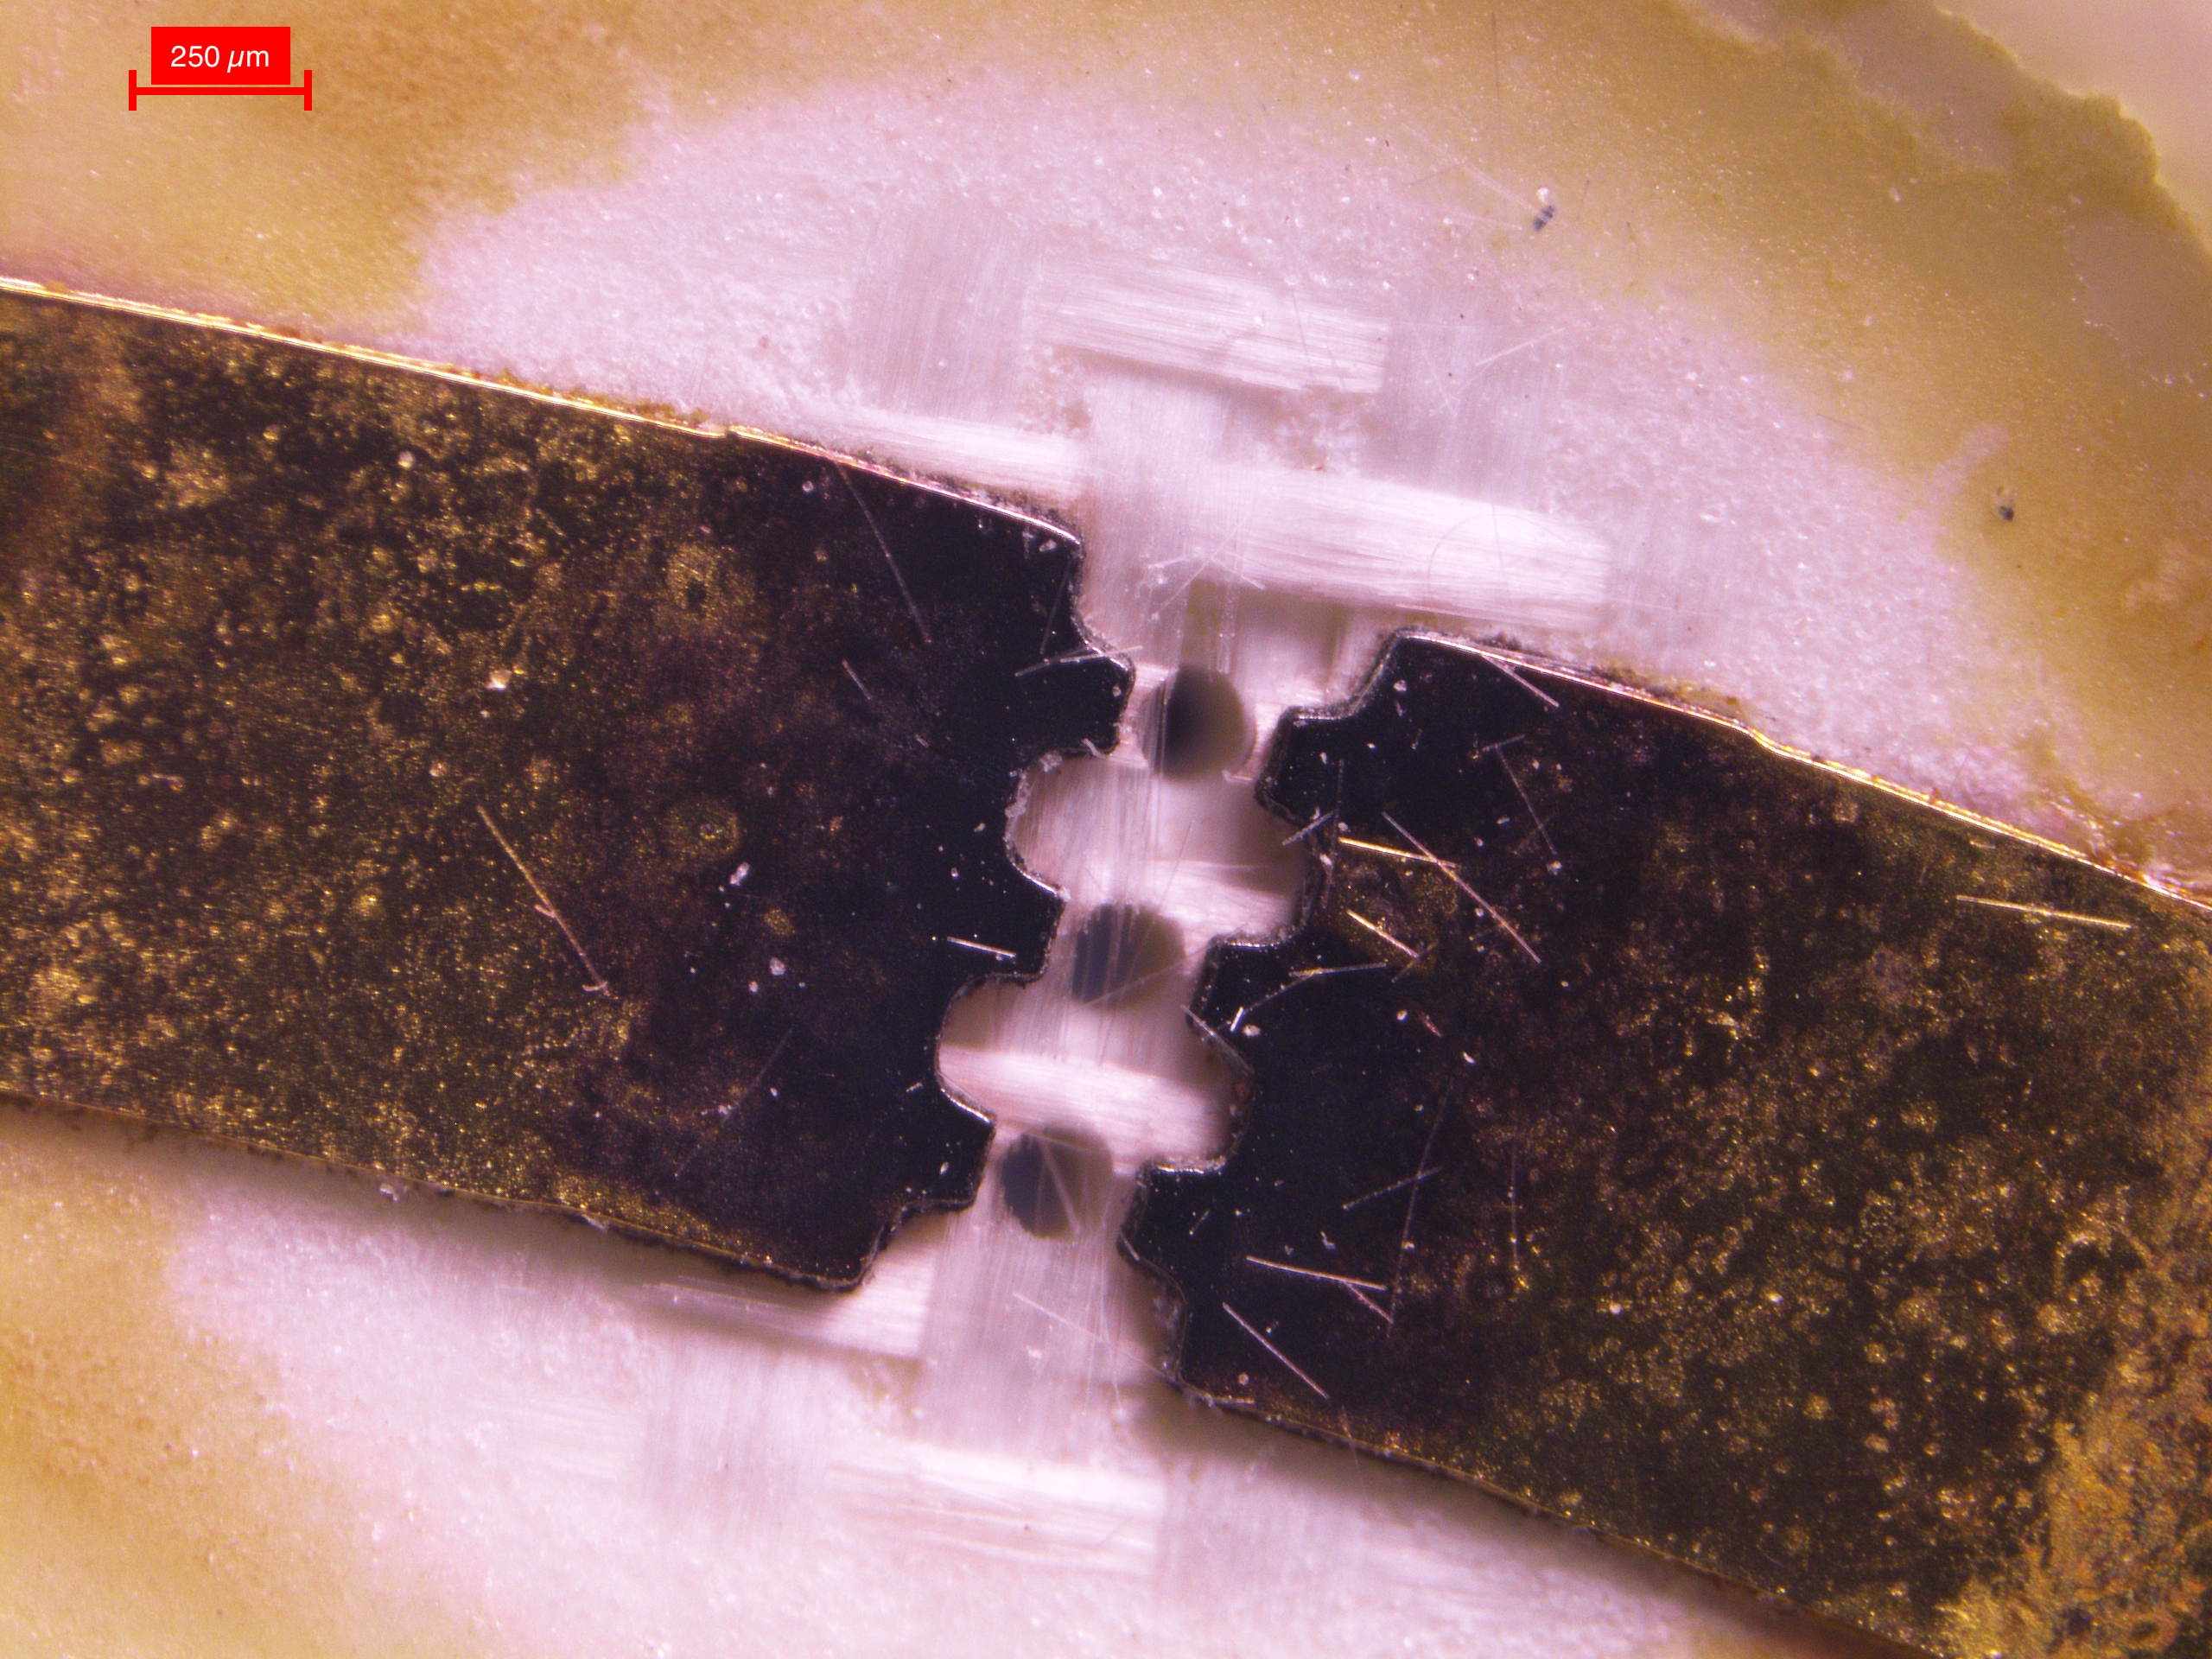
\includegraphics[width=0.8\textwidth]{chapter_6/figures/carbon_deposition.png}
        \caption{}
        \label{fig:carbon_deposition}
    \end{subfigure}
    \vfill
    \begin{subfigure}[b]{\textwidth}  
        \centering 
        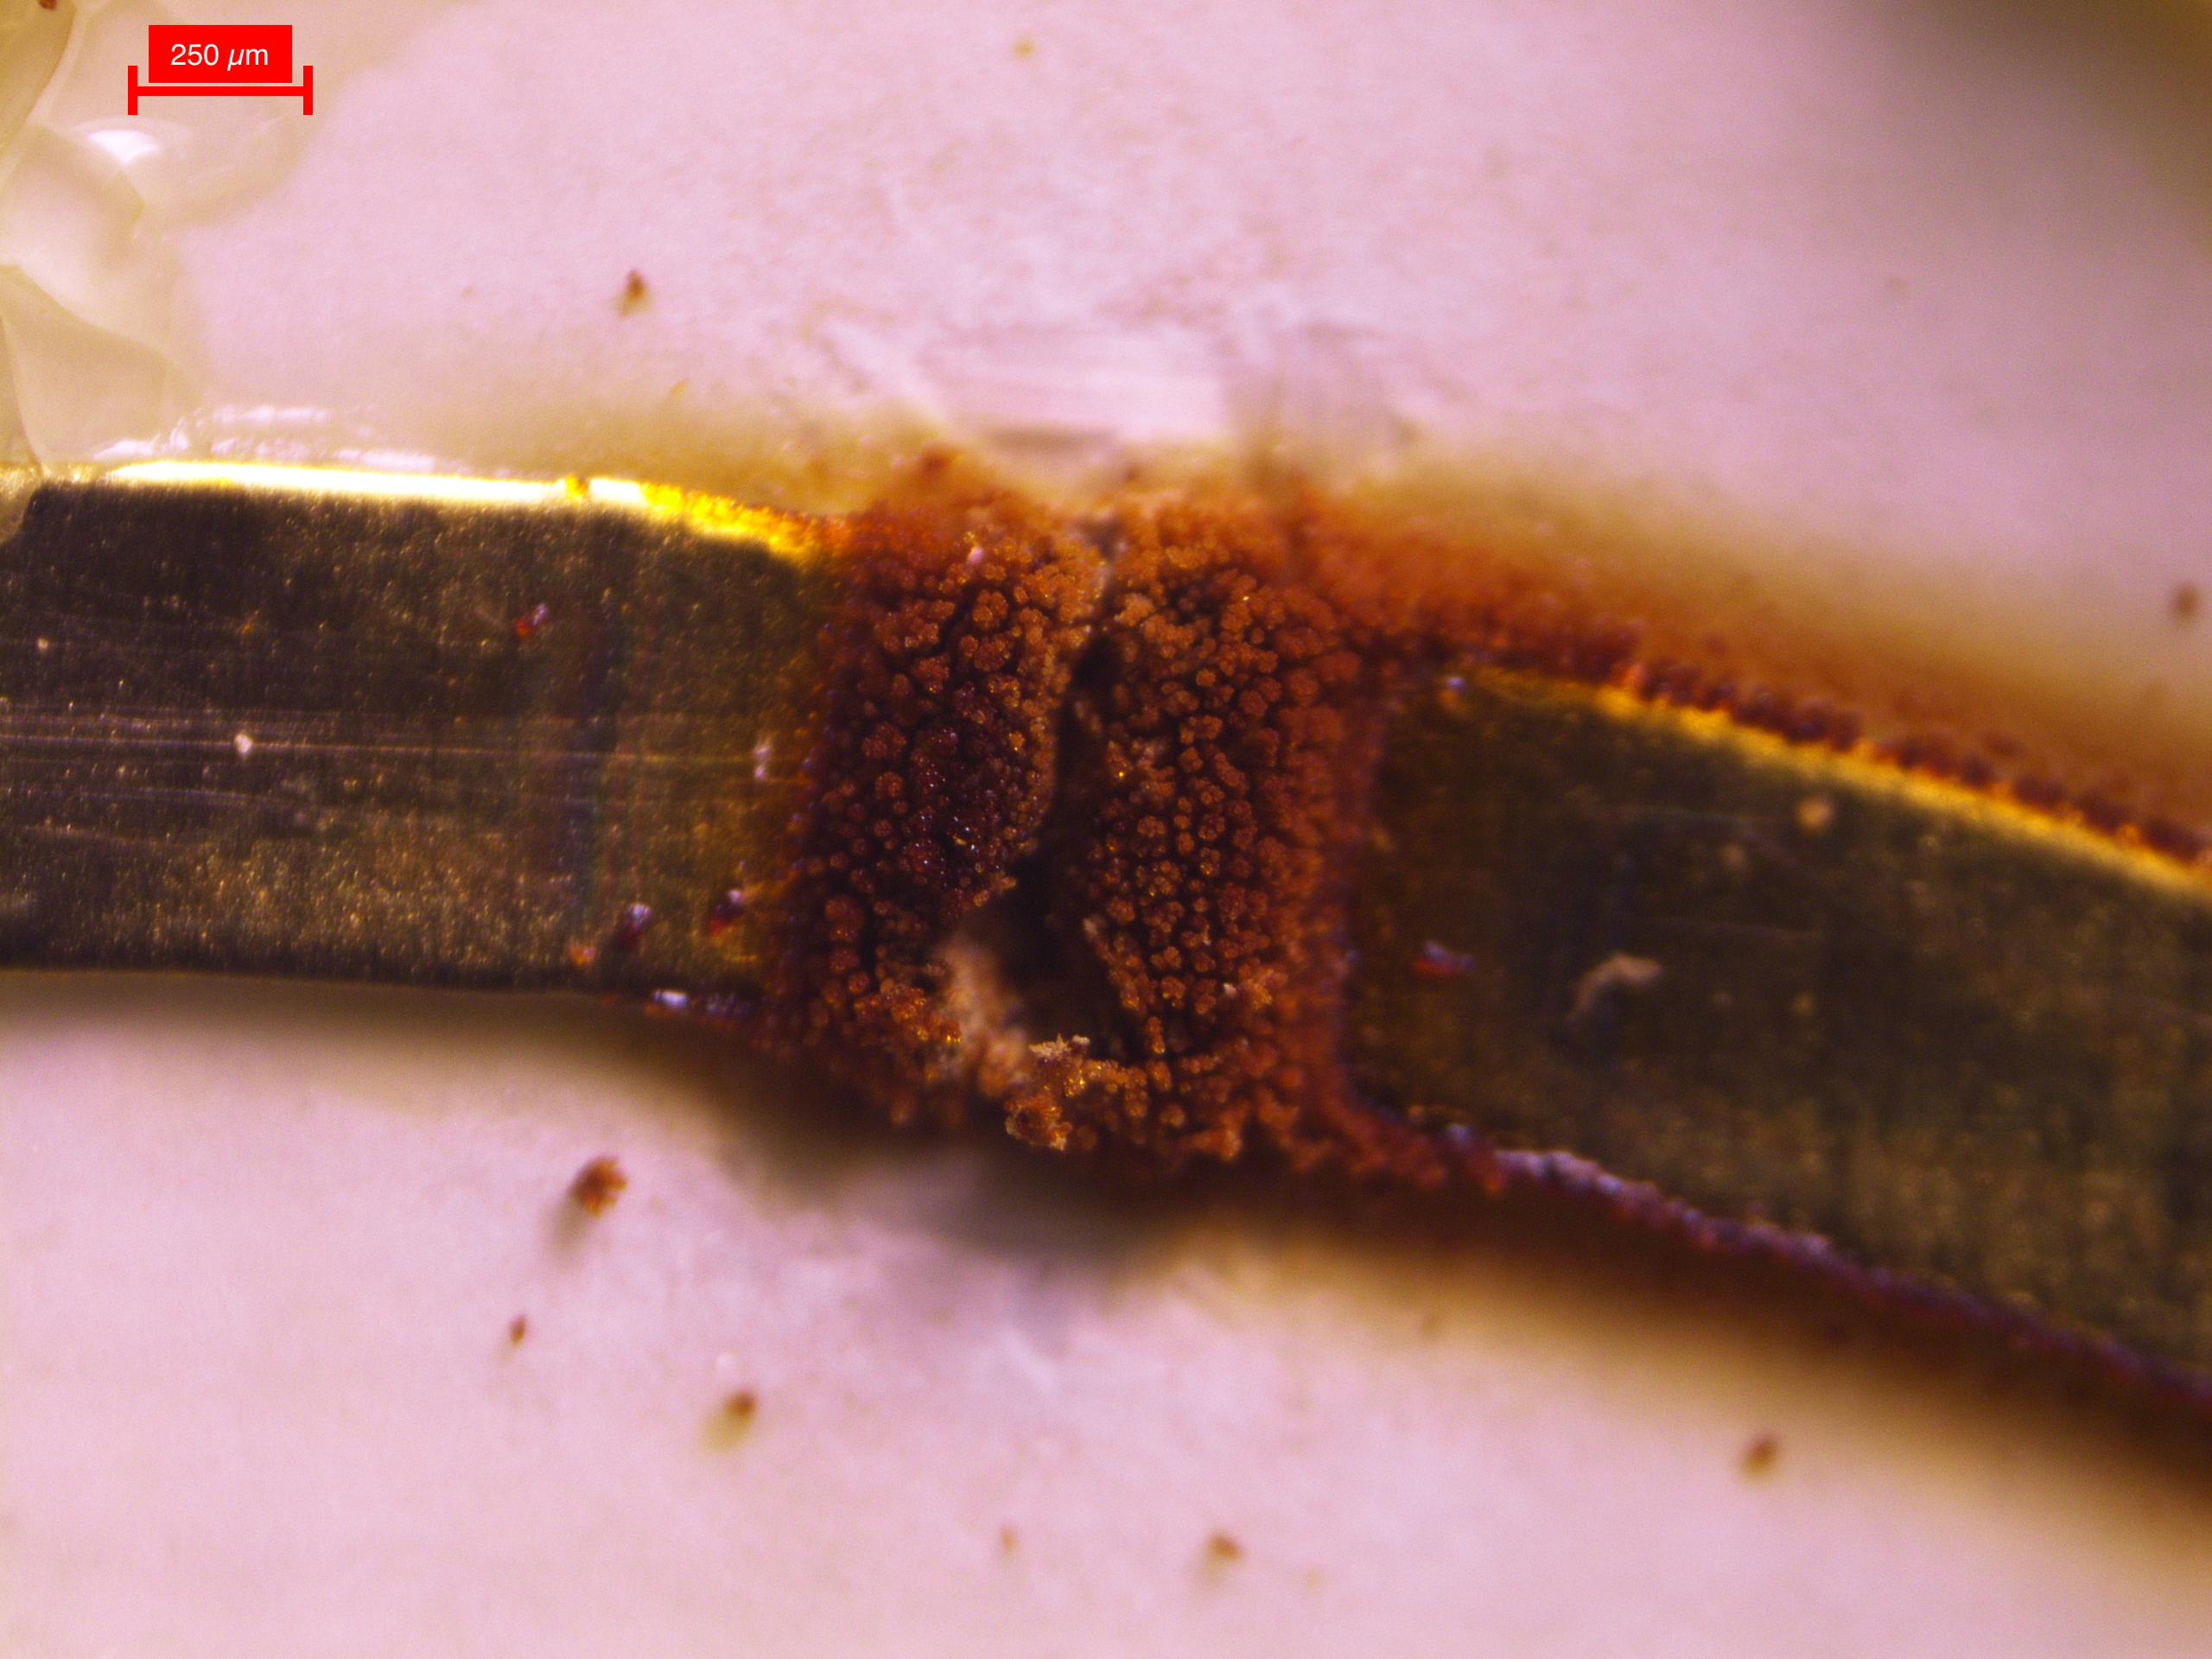
\includegraphics[width=0.8\textwidth]{chapter_6/figures/organic_solvent_deposition.png}
        \caption{}
        \label{fig:organic_solvent_deposition}
    \end{subfigure}
    \caption{\small A comparison between pure carbon deposition (a) and potentially organic solvent deposition  (b) on the SRR electrodes.} 
    \label{fig:deposition_comparison}
\end{figure}


The explantation for why the closed gas loop configuration performed worst was primarily due to contamination of the plasma with the organic solvents used. This included any residual acetonitrile not condensed by the direct-contact condenser and any cooling liquid from the condenser that was kicked up by bubbling the gas through it. This would explain why as time went on, the reactor performed worse in this configuration. This was not necessarily from cumulative accumulation of the organic solvents in the gaseous phase, as this would be limited by the partial pressure of the compound at a given temperature. Instead, this was due to the solvent deposition on the electrodes of the SRR, and as some of the solvent molecules came out of the gas phase, they were immediately replaced by new molecules. 

This deposition was detrimental for two reasons. The first is that it obviously blocks the very small orifice of the SRR jet. But the other, more pernicious issue is that the deposited solvent behaves resistively, and since the power going into the SRR PCB remained constant at 10 W, there was less power going into sustaining the plasma. Less power means, fewer ionising collisions, which in turn reduces the amount of atomic oxygen available for creating the epoxide.

Nonetheless, the fact that a closed gas loop configuration works is a massive step forward as it proves that it is possible to recirculate the feed gas to save on the usage of inert helium gas. More on the feasibility, specifically on the cost of this method, is discussed in the next section.

\section{Cost analysis of recirculating the feed gas}

As previously mentioned, the use of helium of as a feed gas is quite expensive. At the time of writing, a 300 Bar (which is equivalent to roughly 225,000 Torr) cylinder of A grade helium (which is a 99.996\% purity rating) by the supplier BOC\footnote{https://www.boconline.co.uk/} cost £1,337. As per the manufacturers data sheet \cite{bocHeliumDS}, this cylinder would have a gas volume of 12.98 m$^3$ or 12,980 L. Note that this is the equivalent volume at 1 atmosphere of pressure with a gas temperature of 15 $\circ$C. Assuming that all the helium gas could be extracted from the cylinder, it would give the helium a cost of 10.3 p/L. Therefore, running an experiment with a steady 250 sccm flow rate of helium in the open gas loop configuration gives a helium usage rate of 15 L/hr and the cost of running this gas per hour would be 154.5 p/hr. 

Over the span of the 3 hour long closed gas loop experiment, the total helium gas usage to top up the system was 240 cm$^3$, or more conveniently 0.24 L. While this value was significantly worse than the results obtained in the end of chapter 5 in the dry plasma system, with a 16 times increase in gas usage over a 1/8 period of original 24 test, it was to be expected. The reason being, there were more parts in the wet plasma system, which simply meant more points at which leaks could occur. Next, looking at the concentration epoxide produced in closed gas loop configuration over the 3 hour run, it took an equivalent of 1.5 hours in the open gas loop configuration to produce the same amount. In that span of time, the open gas loop experiment used 20.4 L of helium. Thus, it can be said that the the closed loop gas configuration saved nearly 94 times the amount of feed gas used in order to achieve the same concentration of epoxide produced. When translated to the cost of helium used, the open gas loop configuration used 210.12p whereas the closed gas loop configuration used 2.47p, which was a saving of £2.08. Note that this was also with the drop off in plasma performance due to contamination, thus could be said to be the worst case scenario. Solving that issue, along with making the total setup more leak proof, would only improve the savings for the closed gas loop configuration.   

The same calculations could be performed for the CO$_2$ gas used. BOC sells a 34 kg CO$_2$ cylinder (with a 99.8\% purity rating) for £63.59. The exact gas volume of the cylinder was not stated on the datasheet \cite{bocCO2DS}, but based on the density of CO$_2$ at room temperature and atmospheric pressure, the calculated gas volume of 17.172 m$^3$ or 17172 L. This meant that CO$_2$ has a cost of 0.37 p/L, and running a 1\% CO$_2$-He gas mixture would give a CO$_2$ usage rate of 0.15 L/hr. The cost of running the CO$_2$ gas per hour would be 0.06 p/hr. Because of how trivial this cost was, it was excluded from the rest of the calculations.

From these calculations, it is obvious that the closed gas loop configuration saves significantly in terms of costs for the feed gas. However, there is a trade off for running these experiments longer which is the cost of electricity. The current price of electricity in the UK is 24.5 p/kWh. Note that this is the cost of electricity for households, businesses would typically pay less though the exact amount varies based on the size of the business and the energy provider. Nevertheless, this illustrates a worst-case scenario for running the experiments. 

While the power required to drive the plasma was only 10 W, in order to drive the plasma, a signal generator and an amplifier were used. The details of the electrical setup can be found in chapter 4, but it is safe to say that the equipment used to drive the plasma certainly used more than 10 W of power. To measure the power consumed by the equipment, a plug-in power monitor was used. The measured power when running the plasma from the signal generator and amplifier were 45 W and 230 W respectively. On top of these two pieces of equipment, there were the MKS mass flow controllers and pressure sensors which drew 168 W in total, the FTIR which drew 80 W, and the pump and heating element for the direct-contact condenser setup that drew 39 W. Thus, the total power usage was 562 W. Running this for 3 hours would equate to 1.686 kWh, which equates to 41.31p of electricity used. Hence, even when factoring electricity usage into the total cost of operation, the closed gas loop configuration saved roughly £1.64. 

Moreover, this is with an unoptimised power setup, as the amplifier and signal generator used was designed to operate at a large range of frequencies. If a custom power supply were built, such as the case with the COST jet, the savings would be even larger. For reference, the power usage of the COST jet power supply was measured to be 49 W. Which means, that the total power usage could be brought down to between 50-60 \% of the current value. Regardless, with the current setup, it can be said that the closed gas loop configuration operates at 20\% the cost of the open gas loop configuration.

